\documentclass[11pt,a4paper]{article}

\usepackage[a4paper,left=2.0cm,right=2.0cm,top=1.55cm,bottom=1.55cm]{geometry}
\usepackage[T1]{fontenc}
\usepackage{lmodern}
\usepackage{graphicx}
\usepackage{xcolor}
\usepackage{array}
\usepackage{tabularx}
\usepackage{ragged2e}
\usepackage{enumitem}
\usepackage{fancyhdr}
\usepackage{tikz}
\usetikzlibrary{positioning,arrows.meta}
\usepackage{tcolorbox}
\tcbuselibrary{breakable}
\usepackage{setspace}

\definecolor{TitleBlue}{RGB}{61,103,154}

\setlength{\parindent}{0pt}
\setlength{\parskip}{0pt}
\renewcommand{\arraystretch}{1.0}

\newcommand{\blueheading}[1]{% 
  {\sffamily\color{TitleBlue}\fontsize{15}{18}\selectfont #1}%
}
\newcommand{\bluebigheading}[1]{% 
  {\sffamily\bfseries\color{TitleBlue}\fontsize{16}{19}\selectfont #1}%
}

% The original document uses thin rectangular answer boxes.
\newtcolorbox{answerbox}{%
  breakable,
  colback=white,
  colframe=black,
  boxrule=0.45pt,
  arc=0pt,
  left=3mm,
  right=3mm,
  top=2.5mm,
  bottom=2.5mm,
  fontupper=\small
}

\newcommand{\memberphoto}[1]{%
  \includegraphics[width=2.5cm,height=3.0cm,keepaspectratio]{#1}%
}

\pagestyle{fancy}
\fancyhf{}
\renewcommand{\headrulewidth}{0pt}
\renewcommand{\footrulewidth}{0pt}
\fancyhead[L]{%
  \sffamily\bfseries\itshape\fontsize{10.5}{12}\selectfont
  DATA STRUCTURES AND C++
}
\fancyhead[R]{%
  \sffamily\bfseries\fontsize{10.5}{12}\selectfont
  PROJECT PROPOSAL
}
\fancyfoot[R]{%
  \itshape\fontsize{10}{12}\selectfont Page \thepage
}
\setlength{\headheight}{14pt}
\setlength{\headsep}{23pt}
\setlength{\footskip}{24pt}

\begin{document}

% =========================================================
% PAGE 1
% =========================================================
\vspace*{4mm}
\bluebigheading{PROJECT AND TEAM INFORMATION}

\vspace{13mm}
\blueheading{Project Title}

\vspace{2mm}
\begin{answerbox}
\begin{center}
\fontsize{10.5}{13}\selectfont
EduTrack: Intelligent Student Performance and Academic Record Management\par
System
\end{center}
\end{answerbox}

\vspace{13mm}
\blueheading{Student / Team Information}

\vspace{2mm}
\noindent
\begin{tabularx}{\textwidth}{|>{\RaggedRight\arraybackslash}p{0.69\textwidth}|>{\centering\arraybackslash}X|}
\hline
\begin{minipage}[t]{\linewidth}
\vspace{1.5mm}
\textit{Team Name:}\\[-1mm]
\textit{Team ID:}
\vspace{0.5mm}
\end{minipage}
&
\begin{minipage}[t]{\linewidth}
\vspace{1.5mm}
EduTrack\\[-1mm]
DSCPP-III-2026-T287
\vspace{1.5mm}
\end{minipage}
\\
\hline
\begin{minipage}[t]{\linewidth}
\vspace{3mm}
\textit{Team member 1 (Team Lead)}\\[2mm]
Mohammad Rayyan Farooqui\\[1.5mm]
Student ID: 2510370176\\[1.5mm]
2510370176@geu.ac.in
\vspace{1.5mm}
\end{minipage}
&
\begin{minipage}[c]{\linewidth}\centering
\memberphoto{member1.jpg}
\end{minipage}
\\
\hline
\begin{minipage}[t]{\linewidth}
\vspace{1.5mm}
\textit{Team member 2}\\[2mm]
Shiv Tyagi\\[1.5mm]
Student ID: 2510370194\\[1.5mm]
2510370194@geu.ac.in
\vspace{1.5mm}
\end{minipage}
&
\begin{minipage}[c]{\linewidth}\centering
\memberphoto{member2.jpg}
\end{minipage}
\\
\hline
\begin{minipage}[t]{\linewidth}
\vspace{1.5mm}
\textit{Team member 3}\\[2mm]
Bhaskar Bahukhandi\\[1.5mm]
Student ID: 2510370009\\[1.5mm]
2510370009@geu.ac.in
\vspace{1.5mm}
\end{minipage}
&
\begin{minipage}[c]{\linewidth}\centering
\memberphoto{member3.jpg}
\end{minipage}
\\
\hline
\begin{minipage}[t]{\linewidth}
\vspace{1.5mm}
\textit{Team member 4}\\[2mm]
Aditya Kukrety\\[1.5mm]
Student ID: 2510012343\\[1.5mm]
2510012343@geu.ac.in
\vspace{1.5mm}
\end{minipage}
&
\begin{minipage}[c]{\linewidth}\centering
\memberphoto{member4.jpg}
\end{minipage}
\\
\hline
\end{tabularx}

\vspace{4mm}
\noindent
\begin{tabularx}{\textwidth}{|p{0.14\textwidth}|X|}
\hline
\textit{Mentor} & Mr. Abhinav Kotnala \\
\hline
\textit{Email} & abhinavkotnala.cse@geu.ac.in \\
\hline
\end{tabularx}

\newpage

% =========================================================
% PAGE 2
% =========================================================
\bluebigheading{PROPOSAL DESCRIPTION (10 pts)}

\vspace{12mm}
\blueheading{Motivation (1 pt)}

\vspace{3mm}
\begin{answerbox}
Managing student academic records can become time-consuming and difficult when the number of students increases. Information such as student details, marks, grades and academic performance may be maintained in separate records, making searching, updating and organizing information more difficult.

A simple and efficient academic record management system is therefore required to make these operations faster and more organized. The proposed system, EduTrack, aims to provide a C++-based solution for maintaining student academic records while also demonstrating the practical application of Data Structures and Algorithms.

The system will allow student details and subject-wise marks to be stored and managed efficiently. It will automate academic calculations such as total marks, percentage and grades. It will also provide searching and sorting capabilities so that student records can be retrieved and organized efficiently.

A major motivation for the project is to go beyond basic record storage. EduTrack will use algorithmic processing to analyze academic performance, identify the top-performing student, generate a dynamic rank list and compare individual performance with the class average.

The project also provides an opportunity to apply concepts studied in Data Structures and C++, including vectors or dynamic arrays, searching, sorting, queues, stacks, Object-Oriented Programming and file handling.

Thus, EduTrack addresses a practical academic record management problem while providing meaningful integration of the concepts learned in the course.
\end{answerbox}

\vspace{7mm}
\blueheading{State of the Art / Current solution (1 pt)}

\vspace{3mm}
\begin{answerbox}
Student academic information is commonly maintained through manual records, spreadsheets, institutional management systems or separate digital files. These methods can be useful for storing information, but several operations still require repetitive manual processing.

For example, searching for a particular student, updating records, calculating percentages, arranging students by performance and preparing rank lists can become increasingly difficult when the number of records grows.

A basic Student Management System can solve some of these problems by storing student details and providing operations such as insertion, searching, updating and deletion. However, a basic record-management approach does not necessarily provide integrated academic performance analysis using Data Structures and Algorithms.

EduTrack proposes an enhanced approach in which student record management is combined with academic processing. Student records can be searched using their Roll Number, while sorting algorithms can arrange students according to marks or percentage.

The sorted records can then be used to generate a dynamic academic rank list. Additional processing can identify the top-performing student, categorize student performance, display subject-wise performance and compare individual performance with the class average.

The project therefore focuses on integrating C++, Object-Oriented Programming and DSA concepts into a single academic record management and analysis system.
\end{answerbox}

\newpage

% =========================================================
% PAGE 3
% =========================================================
\bluebigheading{PROPOSAL DESCRIPTION (10 pts)}

\vspace{12mm}
\blueheading{Project Goals and Milestones (2 pts)}

\vspace{3mm}
\begin{answerbox}
The primary goal of EduTrack is to develop an efficient C++-based student academic record management system that combines student record management with academic processing, searching, sorting, ranking and performance analysis.

The major goals of the project are:
\begin{enumerate}[leftmargin=7mm,itemsep=1.5pt,topsep=2pt,parsep=0pt]
\item Develop a C++-based student academic record management system.
\item Store student details and subject-wise marks efficiently.
\item Automatically calculate total marks, percentage and grades.
\item Provide searching functionality for student records.
\item Allow student records to be updated and deleted.
\item Apply suitable sorting techniques to organize students according to marks or percentage.
\item Generate a dynamic academic rank list.
\item Identify the top-performing student.
\item Categorize students according to their academic performance.
\item Display subject-wise performance of students.
\item Compare individual student performance with the class average.
\item Maintain permanent student records using C++ file handling.
\item Demonstrate meaningful integration of Object-Oriented Programming and Data Structures and Algorithms.
\end{enumerate}

\textbf{Initial Milestones}
\begin{enumerate}[leftmargin=7mm,itemsep=1.5pt,topsep=2pt,parsep=0pt]
\item Problem identification and formulation.
\item Background research and requirement analysis.
\item Identification of major system features.
\item Design of the proposed system workflow.
\item Mapping of C++ OOP and DSA concepts to individual system modules.
\item Development of the basic C++ implementation.
\item Implementation of student record operations.
\item Integration of searching and sorting algorithms.
\item Implementation of academic performance analysis.
\item Integration of file handling for permanent storage.
\item Testing and debugging.
\item Final evaluation and refinement.
\end{enumerate}
\end{answerbox}

\vspace{7mm}
\blueheading{Project Approach (3 pts)}

\vspace{3mm}
\begin{answerbox}
The proposed EduTrack system will be developed as a modular C++ application. The development process will begin with student information such as Roll Number, Name, Branch and Semester, along with marks for different subjects.

A Student class will be used to represent individual student records. Object-Oriented Programming principles will be used to organize the system into appropriate classes and functions. Encapsulation will help maintain controlled access to student information, while constructors can be used to initialize student objects.

Student records will be maintained using suitable data structures, particularly vectors or dynamic arrays. These structures will allow multiple student records to be stored and processed dynamically.

The academic processing module will calculate total marks, percentage and grades. Searching techniques will be used to retrieve student records efficiently.

Linear Search can be used for straightforward searching, while Binary Search can be applied when the records are maintained in a suitable sorted order.

Sorting algorithms will be used to arrange students according to marks or percentage. The sorted data can then be used to generate a dynamic academic rank list and identify the top-performing student.

The system will also perform basic academic analysis. This will include student performance categorization, subject-wise performance and comparison between individual student performance and the class average.

Queue and Stack concepts can also be incorporated where appropriate. A Queue can represent students waiting for processing or verification, whereas a Stack can be used for maintaining recently performed operations.

Permanent storage will be implemented using C++ file handling and the \texttt{fstream} library. This will allow student records to be written to files and retrieved when the program is executed again.

\textbf{Technology and Concept Stack}
\begin{itemize}[leftmargin=7mm,itemsep=1.5pt,topsep=2pt,parsep=0pt]
\item C++ programming language.
\item Object-Oriented Programming.
\item Classes and Objects.
\item Encapsulation.
\item Constructors.
\item Inheritance and Polymorphism where required.
\item Vector / Dynamic Array.
\item Queue.
\item Stack.
\item Linear Search.
\item Binary Search.
\item Sorting Algorithms.
\item Algorithmic processing.
\item C++ File Handling using \texttt{fstream}.
\end{itemize}

\textbf{Development Methodology}

The development will follow the stages of problem identification, background research, requirement analysis, system design, DSA and OOP mapping, implementation, testing, debugging and evaluation.
\end{answerbox}

\newpage

% =========================================================
% PAGE 5
% =========================================================
\blueheading{System Architecture (High Level Diagram)(2 pts)}

\vspace{10mm}
\begin{answerbox}
The proposed EduTrack system consists of several connected modules. Student information first enters the Student Input module and is then transferred to the Student Record Management module.

The stored information is processed by the Academic Processing module, which calculates marks, percentage and grades. Search and Sorting modules process the records to retrieve students and organize them according to their academic performance.

The Performance Analysis module uses the processed information to generate rankings, identify top-performing students and compare individual performance with the class average.

The File Storage module provides permanent storage of student records and allows information to be retrieved in future program executions.
\end{answerbox}

\vspace{8mm}
\begin{center}
\begin{tikzpicture}[
  box/.style={draw, rounded corners=2pt, minimum width=3.0cm, minimum height=0.95cm, align=center, font=\fontsize{9}{10}\selectfont},
  arrow/.style={-{Latex[length=2mm]}, thick}
]
\node[box] (a) {Student\\Input};
\node[box,right=0.55cm of a] (b) {Student Record\\Management};
\node[box,right=0.55cm of b] (c) {Academic\\Processing};
\node[box,right=0.55cm of c] (d) {Search \&\\Sorting};
\node[box,right=0.55cm of d] (e) {Performance\\Analysis};
\node[box,below=1.25cm of c] (f) {File\\Storage};

\draw[arrow] (a)--(b);
\draw[arrow] (b)--(c);
\draw[arrow] (c)--(d);
\draw[arrow] (d)--(e);
\draw[arrow] (c)--(f);
\draw[arrow] (f)--(e);
\end{tikzpicture}
\end{center}

\vspace{8mm}
\begin{answerbox}
\textbf{System Components}

\begin{itemize}[leftmargin=7mm,itemsep=2pt,topsep=3pt,parsep=0pt]
\item \textbf{Student Input Module:} Accepts student details and subject-wise marks.
\item \textbf{Student Record Management:} Handles creation, display, updating, searching and deletion of student records.
\item \textbf{Academic Processing:} Calculates total marks, percentage and grades.
\item \textbf{Search and Sorting:} Uses searching and sorting algorithms for efficient record organization and retrieval.
\item \textbf{Performance Analysis:} Generates rankings, identifies top performers and compares student performance with class-level performance.
\item \textbf{File Storage:} Maintains student records permanently using C++ file handling.
\end{itemize}
\end{answerbox}

\newpage

% =========================================================
% PAGE 6
% =========================================================
\blueheading{Project Outcome / Deliverables (1 pts)}

\vspace{8mm}
\begin{answerbox}
The proposed EduTrack system is expected to provide a structured and efficient approach for managing and analyzing student academic records.

The major expected outcomes and deliverables are:
\begin{enumerate}[leftmargin=7mm,itemsep=1.5pt,topsep=2pt,parsep=0pt]
\item A functional C++ student academic record management system.
\item Student record creation, display, searching, updating and deletion functionality.
\item Automated calculation of total marks, percentage and grades.
\item Efficient searching of student records.
\item Sorting of students according to academic performance.
\item A dynamic academic rank list.
\item Identification of the top-performing student.
\item Academic performance categorization.
\item Subject-wise student performance information.
\item Comparison of individual student performance with the class average.
\item Permanent storage and retrieval of student records using C++ file handling.
\item Practical demonstration of C++ Object-Oriented Programming.
\item Practical application of Data Structures and Algorithms to a real-world academic management problem.
\end{enumerate}

The final project is expected to demonstrate that DSA concepts can be used not only for theoretical problems but also for organizing, searching, processing and analyzing real-world academic information.
\end{answerbox}

\vspace{7mm}
\blueheading{Assumptions}

\vspace{3mm}
\begin{answerbox}
The proposed system assumes that valid student information and subject-wise marks will be provided as input.

Each student is assumed to have a unique Roll Number that can be used for identification and searching.

The grading and percentage calculation rules used by the system are assumed to be defined before implementation.

It is assumed that users entering or modifying student records will provide information in the expected format.

The current project is primarily intended as an academic project for demonstrating C++ Object-Oriented Programming and Data Structures and Algorithms. Advanced institutional database integration, authentication and large-scale deployment are outside the current proposed scope.
\end{answerbox}

\newpage

% =========================================================
% PAGE 7
% =========================================================
\blueheading{References}

\vspace{8mm}
\begin{answerbox}
The following categories of resources will be used during the development and documentation of the EduTrack project:

\begin{enumerate}[leftmargin=7mm,itemsep=2pt,topsep=3pt,parsep=0pt]
\item C++ programming and Object-Oriented Programming reference materials.
\item Data Structures and Algorithms reference materials.
\item C++ Standard Library documentation.
\item Documentation related to C++ vectors and dynamic arrays.
\item Documentation and reference material for searching and sorting algorithms.
\item C++ file handling and \texttt{fstream} documentation.
\item Academic management system reference material consulted during the problem analysis and proposal development.
\item Course material related to Data Structures and C++.
\end{enumerate}

\vspace{6mm}
\textbf{Technical References}

\begin{itemize}[leftmargin=7mm,itemsep=2pt,topsep=3pt,parsep=0pt]
\item C++ Standard Library documentation.
\item Data Structures and Algorithms course resources.
\item C++ Object-Oriented Programming reference resources.
\item File handling and \texttt{fstream} documentation.
\end{itemize}
\end{answerbox}

\end{document}
